\documentclass[tikz,border=8pt]{standalone}
% Shared look for every TikZ diagram. Load with \input{../../tools/tikz-style.tex}
\usepackage[T1]{fontenc}
\usepackage{lmodern}
\renewcommand{\sfdefault}{lmr}  % diagrams use the same serif as the text
\usetikzlibrary{arrows.meta, positioning, shapes.geometric, calc, fit, backgrounds}
\definecolor{cblue}{HTML}{4C78A8}
\definecolor{corange}{HTML}{F58518}
\definecolor{cgreen}{HTML}{54A24B}
\definecolor{cred}{HTML}{E45756}
\definecolor{cpurple}{HTML}{B279A2}
\definecolor{cgrey}{HTML}{6B6B6B}
\tikzset{
  every picture/.style={font=\sffamily, line width=1.2pt},
  box/.style={draw=#1, fill=#1!12, rounded corners=4pt, align=center, inner sep=7pt, minimum height=1.1cm},
  box/.default=cgrey,
  arrow/.style={-{Stealth[length=3mm]}, draw=cgrey, line width=1.4pt},
  title/.style={font=\sffamily\bfseries\Large},
  note/.style={font=\sffamily\small, text=cgrey, align=center},
}
\AtBeginDocument{\hyphenpenalty=10000 \exhyphenpenalty=10000}

% A car pulling one trailer, seen from above. Car heading theta_0 = 40 deg, trailer heading theta_1 = 10 deg,
% hitch at the middle of the car's rear axle, hitch length d_1 from the hitch to the middle of the trailer's axle.
\begin{document}
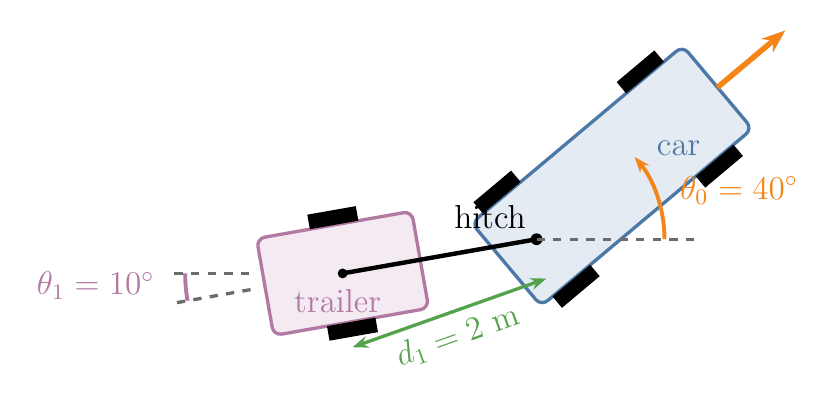
\begin{tikzpicture}[scale=1.25, every node/.append style={font=\large}]
  \coordinate (H) at (0,0);                       % hitch = middle of the car's rear axle
  \coordinate (T) at ({-2*cos(10)},{-2*sin(10)}); % middle of the trailer's axle (d_1 = 2)
  % car
  \begin{scope}[shift={(H)}, rotate=40]
    \draw[cblue, fill=cblue!15, rounded corners=3pt] (-0.4,-0.55) rectangle (2.4,0.55);
    \foreach \xx in {0,1.9} { \fill[black] (\xx-0.25,0.55) rectangle (\xx+0.25,0.7); \fill[black] (\xx-0.25,-0.7) rectangle (\xx+0.25,-0.55); }
    \draw[-{Stealth[length=3mm]}, corange, line width=2pt] (2.4,0) -- (3.3,0);
    \node[cblue] at (1.7,-0.22) {car};
  \end{scope}
  % trailer
  \begin{scope}[shift={(T)}, rotate=10]
    \draw[cpurple, fill=cpurple!15, rounded corners=3pt] (-0.8,-0.5) rectangle (0.8,0.5);
    \fill[black] (-0.25,0.5) rectangle (0.25,0.65); \fill[black] (-0.25,-0.65) rectangle (0.25,-0.5);
    \node[cpurple] at (-0.1,-0.27) {trailer};
  \end{scope}
  \draw[black, line width=1.6pt] (T) -- (H);
  \fill[black] (H) circle (0.06); \fill[black] (T) circle (0.05);
  \node[above left] at (H) {hitch};
  \draw[{Stealth[length=2mm]}-{Stealth[length=2mm]}, cgreen, line width=1.2pt] ($(T)+(0.1,-0.75)$) -- ($(H)+(0.1,-0.4)$) node[midway, below, sloped] {$d_1 = 2$ m};
  % headings
  \draw[cgrey, dashed] (H) -- ++(1.6,0);
  \draw[corange, line width=1.4pt, -{Stealth[length=2mm]}] ($(H)+(1.3,0)$) arc (0:40:1.3);
  \node[corange, right] at ($(H)+(1.35,0.5)$) {$\theta_0 = 40^\circ$};
  \draw[cgrey, dashed] ($(T)+(-0.95,0)$) -- ++(-0.8,0);
  \draw[cgrey, dashed] ($(T)+({-0.95*cos(10)},{-0.95*sin(10)})$) -- ++({-0.8*cos(10)},{-0.8*sin(10)});
  \draw[cpurple, line width=1.4pt] ($(T)+(-1.6,0)$) arc (180:190:1.6);
  \node[cpurple, left] at ($(T)+(-1.8,-0.12)$) {$\theta_1 = 10^\circ$};
\end{tikzpicture}
\end{document}
